\documentclass[a4paper,12pt,numbered,print,index]{report/thesisFormat}
\usepackage{blindtext}
\usepackage{mathtools}
\usepackage{amssymb}
\usepackage{tikz}
\usepackage{multirow}
\usepackage[T1]{fontenc}
\usetikzlibrary{shapes,arrows}
\usepackage[parfill]{parskip}
\urlstyle{same}
\linespread{1.5}
\let\oldemptyset\emptyset
\let\emptyset\varnothing

\usepackage{listings}
\usepackage{courier}
\definecolor{mygreen}{rgb}{0,0.6,0}
\definecolor{mygray}{rgb}{0.5,0.5,0.5}
\definecolor{mymauve}{rgb}{0.58,0,0.82}

\lstset{ %
  backgroundcolor=\color{white},   % choose the background color; you must add \usepackage{color} or \usepackage{xcolor}
  basicstyle=\tiny,                 % the size of the fonts that are used for the code
  breakatwhitespace=false,         % sets if automatic breaks should only happen at whitespace
  breaklines=true,                 % sets automatic line breaking
  captionpos=b,                    % sets the caption-position to bottom
  commentstyle=\color{mygreen},    % comment style
  extendedchars=true,              % lets you use non-ASCII characters; for 8-bits encodings only, does not work with UTF-8
  frame=single,	                   % adds a frame around the code
  keepspaces=true,                 % keeps spaces in text, useful for keeping indentation of code (possibly needs columns=flexible)
  keywordstyle=\color{blue},       % keyword style
  language=Python,                 % the language of the code
  numbers=left,                    % where to put the line-numbers; possible values are (none, left, right)
  numbersep=5pt,                   % how far the line-numbers are from the code
  numberstyle=\tiny\color{mygray}, % the style that is used for the line-numbers
  rulecolor=\color{black},         % if not set, the frame-color may be changed on line-breaks within not-black text (e.g. comments (green here))
  showspaces=false,                % show spaces everywhere adding particular underscores; it overrides 'showstringspaces'
  showstringspaces=false,          % underline spaces within strings only
  showtabs=false,                  % show tabs within strings adding particular underscores
  stepnumber=2,                    % the step between two line-numbers. If it's 1, each line will be numbered
  stringstyle=\color{mymauve},     % string literal style
  tabsize=2,	                   % sets default tabsize to 2 spaces
  title=\lstname                   % show the filename of files included with \lstinputlisting; also try caption instead of title
}


\usepackage{graphicx}
\usepackage{caption}
\usepackage{subcaption}

\graphicspath{ {report/images/} }
\newgeometry{inner=2.8cm, outer=3cm, top=3cm, bottom=3cm}

% for roman pages

\newenvironment{romanpages}{
  \setcounter{page}{1}
  \renewcommand{\thepage}{\roman{page}}}
{\newpage\renewcommand{\thepage}{\arabic{page}}}

% ************************ Thesis Information & Meta-data **********************
%% The title of the thesis
\title{\textit{Linear Programming to Solve\\Vehicle Routing Problem}}

%% Subtitle (Optional)
\subtitle{\textit{A Project on Route Optimisation and Analysis of Linear Programming Tools}}

%% The full name of the author
\author{Muhammad Rafdi}

%% Department (eg. Department of Engineering, Maths, Physics)
\dept{Department of Computer Science}

%% University and Crest
\university{University College London}
% Crest minimum should be 30mm.
\crest{
\includegraphics[width=0.45\textwidth]{ucl-logo.jpg}}

%% Full title of the Degree
\degreetitle{BSc Computer Science}

\college{Supervisor: Dr Daniel Hulme}

%% Submission date
% Default is set as {\monthname[\the\month]\space\the\year}
\degreedate{29 April 2016}

\begin{document}

\begin{romanpages}

\begin{titlepage}
  \maketitle
\end{titlepage}

\begin{abstract2}

    Linear programming (LP) is a method to find the optimal solution to combinatorial optimisation problems.
    In this project, we will be using linear programming to solve an instance of a vehicle routing problem (VRP) and
     analyse the performance of three different LP tools: Gurobi, or-tools and
    Optaplanner. Our goal is to be able to find an optimal solution to the problem and analyse the performance and the features
    of the chosen tools.

    First, we create LP formulations: the capacitated vehicle routing problem (CVRP) and the capacitated
     vehicle routing problem with time windows (CVRPTW). Then, we carry out performance
    analysis of the LP tools using the benchmark and test datasets. Finally, we choose a tool based
    on the performance analysis and find the optimal solution to the two LP formulations.

    Our analysis conclude that Optaplanner is the ideal tool for this problem as Gurobi is impractical to use
     and or-tools produce very inefficient solutions to VRP instances. Using
    Optaplanner, we have obtained an optimal solution that uses 8 vehicles with capacity of 29 and yield eucledian
    distances of 10.27 and 10.49 for CVRP and CVRPTW model respectively.

   \vspace{1.5cm}
   \textbf{Keywords} : Linear Programming, Vehicle Routing Problem, Performance Analysis, Gurobi, Optaplanner, or-tools

\end{abstract2}

% set page number

\setcounter{page}{1}

\tableofcontents

\listoffigures

\listoftables

\end{romanpages}

% chapter 1
\chapter{Introduction}
Linear Programming is a mathematical method to find an optimal value of a function in a linear system under a set of
constraints. This method has been around since the 19th century, but it was not fully developed until the World War 2,
where it was used for resources planning. Since its conception, this method has been widely used to solve problems
in Applied Mathematics and Operations Research (OR). Along with the advancement of computing, companies can now increase their
decision making capabilities with efficient technique of linear programming and significant computational power.

Linear programming is used to model to many combinatorial problems, such as vehicle routing.
The vehicle routing problem is a common problem that is commonly observed in logistics.
It is a special instance of the famous traveling salesperson problem in which the tour of
all 'cities' in the given graph into several parts, subject the availability of resources.

In this project, we will conduct an Operations Research study by using linear programming to find the optimal routes of an instance of a vehicle routing
problem. We will use three linear programming tools to arrive at a solution and compare and contrast the results of each one of them.

\section{Project Motivation}
Linear programming has allowed organisations to optimise many aspects its operations. In many occasions, the problem involves
finding the optimal combination of input that yields the greatest output. Amongst the many problems,
vehicle routing is one of them. Many studies have been carried out on this problem due to its role in minimising operational
costs of companies, especially in their logistics department. Logistic plays a significant role in many businesses and it is one of the major
driving force of the economy. In the UK alone, Logistics and Posts Sector is worth approximately
\pounds55bn to the economy and comprises 5 percent of the GDP\footnote{According to a logistics report by PWC }.
In the US, the cost attributed to logistics rose up to US\$1.45 trillion in 2014, an increase of 3.1 percent from the previous year.
These figures are likely to increase given the increasingly globalised economy. Thus, minimising operational costs will not only make companies
more competitive, but it will also increase their profits.

In this project, we want to simulate a scenario where we can optimise
a problem to minimise cost in a fictional delivery company DFFS. We will demonstrate how optimisation can help them solve a vehicle
routing they face.

Aside from financial benefits, the vehicle routing problem is an interesting problem to the mathematically and computationally apt individuals.
There are wide variety of algorithms that can be used to approximate the optimal solution.

A study on the comparison of solvers has been done before in this paper. However, it does not include other open souce LP tools
such as or-tools and Optaplanner, both of which contains their own unique engine to solve LP problems. It will be useful to see the comparison
of different tools as it will help OR analysts to decide which tool is the best for them given their current needs. We have chosen the 3 tools mentioned
because they are relatively popular tools used in the industry there that is relatively well documented and
has an easy to use APIs in various programming languages including Python, the language that we use in this project. Most importantly, they have not
been compared alongside one another.

\section{Goals and Scope of Project}
We have identified a few goals to benchmark this project and a scope to limit the discussions that may have been related to this project. The goals are as
follows:
\begin{enumerate}
\item To thoroughly understand linear programming method to solve optimisation problems.
\item To build a mathematical model of the vehicle routing problem based on the given dataset.
\item Obtain the optimised results (the minimum distance and the paths) using the chosen tools.
\item Compare and contrast the results and the usage of those tools.
\end{enumerate}

Creating novel algorithms for optimisation problems is hard and requires years of experience in Algorithms.
Implementing linear programming solver is also difficult and it requires very high level of software engineering expertise, in addition to
the algorithmic knowledge mentioned. For these reasons, we will not be attempting to create new algorithms or implement linear programming solvers to solve
the vehicle routing problem. Instead we will model the VRP instance using softwares and algorithms that are already available.
In addition, other methods that can be used to solve this problem such as \textit{genetic programming} and \textit{dynamic programming} will
not be covered in this project.

\section{Methodology}
Peforming the calculations for linear programming is not as hard as it used to be given the availability of computing power that we have today.
In this project we will be using three applications: Gurobi, OR Tools by Google and Optaplanner to retrieve the optimal solution. Each of them
contains their own implementation of \textbf{linear programming solver}, a program that can solve linear programming problems. We model them
in a form that can be solved by these solvers and used the solvers to obtain the solution.

This project will be carried out in seven steps, as per the steps taken in a typical OR study:

\begin{enumerate}
\item Define the problem in a given system and formulate it into a linear program. A linear program is a problem that can be solved
using linear programming. In this step, the objective and the constraints of the system is studied thoroughly to ensure
that the program models the given problem correctly.
\item Collect the data that represents the problem at hand and estimated the parameters that are required to produce
the optimal result.
\item Create the mathematical models of the given problem. We will use standard linear programming notation to build these models. This is
also the step in which we implement the linear program using the chosen softwares.
\item Verify that the model is correct. We achieve this by running the implemented linear program through a benchmark dataset with known solution.
\item Select suitable alternative. We may not always get the desired answer, due various reasons such as limited timescale and computing resources.
In this case, we want to select an alternative objectives that will be useful to the parties involved.
\item Run the given problem in the models that we have build and record their result and performance. We may need to go back to step 1 if the results obtained
are not satisfactory.
\item Provide recommendations to the parties involved based on the results obtained.
\end{enumerate}

For comparing the performance of different linear programming tools, we use a 60 node CVRP model. Time limit of 5 minutes is imposed
when running the model on all tools. The optimal distances obtained using each tools will be recorded and compared. In addition, the usage
of the tools will also be discussed.

We use a lot of terminologies interchangeably here such as blah blah blah. This serves as a heads up to the reader... more explanation needed here..

\section{Outline}
In chapter 2, we will elaborate the underlying theory behind linear programming and its state of the art.
The vehicle routing problem will be discussed in detail in chapter 3. The implentation of linear programming to solve the vehicle routing problem will be
discussed in chapter 4, followed by the results in chapter 5. Finally, I will conclude the results and identify potential future works
of this project in chapter 6.

% chapter 2
\chapter{Context}
In this chapter, we will discuss the related works and the relevant concepts that will help the reader understand the ideas
mentioned in this project.

\section{Related Works}
A few studies on the comparison of constraint programming solvers have been done before.
Meindl et al (2012) \cite{Meindl2012} conducted a study on the analysis of popular commercial and open source solvers and concluded
that IBM's CPLEX\footnote{See \url{http://www-01.ibm.com/software/commerce/optimization/cplex-optimizer/}} has the best performance,
followed by Gurobi\footnote{See \url{http://www.gurobi.com}}. Hakan (2012) \cite{Hakan2012} analysed the features of
LP Solvers, including or-tools\footnote{See \url{https://developers.google.com/optimization/}}.
 He stated that or-tools has a lot of advantages such as easy of modelling problems and
active user community. Gurobi Optimization also have carried out comparative study on its tools against other open
source solvers \cite{gurobi:solvers}. The study concludes that Gurobi outperforms the other solvers mentioned.

\section{Linear Programming}
Linear programming (LP) is a mathematical method to obtain the optimal solution of a function in a linear system under set of constraints
imposed on its variables. It is a method commonly used in solving combinatorial optimisation problems in applied mathematics and operations research.
A problem is considered a linear program when all of its mathematical relationship are linear \cite{APMBradley}.
The word 'programming' is not to be confused with the term used in computer science,
in which concerns with creating instructions for computers to execute. A linear
program consists of three entities \cite{LPChvatal,ILPCoursera}:
\begin{enumerate}
\item \textbf{Decision variables} - These are the entities that can be controlled by the decision maker.
\item \textbf{Objective function} - This is the function that, given the optimal input, outputs the optimal value.
In most cases, it is to find the minimum or the maximum value.
\item \textbf{Variable constraints} - These are the restrictions that are imposed on the decision variables. There are two types
of constraints: hard and soft. Hard constraints are constraints cannot be violated at all cost, whereas soft constraints may be
violated, but should be observed wherever possible.
\end{enumerate}

To fully understand LP, it is best to look at an example: Bob is competing in
an eating contest that lasts one hour where the objective is to accumulate as much points as possible by eating a combination of hotdogs and burgers.
For each burger and hotdog that Bob eats, he will get 5 and 4 points respectively. It takes him 3 minutes to finish a burger and
2 minutes to finish a hotdog. Bob can consume 25 food items before his appetite reaches its limit.

Based on the scenario above, we can model this problem in the form of a linear program by following these steps:
\begin{itemize}
\item \textbf{Step 1}: Identify the decision variables. Let \(x\) be the number of hotdogs and \(y\) be the number
of burgers eaten by Bob.
\item \textbf{Step 2}: Determine the objective function. In this scenario, we want to determine the highest possible
points that Bob can achieve in the competition. This can be represented by the equation \(z = 4x + 5y\), where
z is the value of the points accumulated in the competition and the coefficients of the variables represent the points achieved by eating respective
food items.
\item \textbf{Step 3}: Determine the constraints. There are 3 constraints in these problem. Firstly, The amount of
food eaten by bob has to be under 60 minutes. This can be represented by the equation \(2x + 3y \leq 60\). Secondly,
Bob's appetite has a limit of 25 food items, which can be modelled with the equation \(x + y \leq 25\). Lastly,
the number of respective food eaten has to be greater than or equal to 0.
\end{itemize}
Putting them together, we have the following linear program:
\[
  \begin{array}{r@{}r@{}l}
    \text{Maximise z =} \quad &{}4x + 5y \\[\jot]
    \text{Subject to}\qquad &{} 2x +   3y &{} \leq 60 \\
    \qquad &{} x +   \phantom{2}y &{} \leq 25 \\
    \qquad &{} x ,   \phantom{2}y &{} \geq 0 \\
  \end{array}
\]
There are two types of solution that can be produced. A feasible solution is a set of variables that satisfies the constraints
of a linear program. An example of a feasible solution for the above solution would be \(x = 25\) and \(y=0\), which yields 100 points.
The goal of the linear program is to achieve optimal solution of the objective function \cite{LPChvatal}. The optimal solution is the best feasible solutions.
For the problem above, the optimal solution is 110 points, which is produced when \(x = 15\) and \(y = 10\). The feasible solutions
are bound within the feasible region marked in green as shown in Figure 2.1. The red region is the infeasible region, where any point that falls within it will not satisfy the
constraints of the linear program. The dimensions of the graph is determined by the number of variables the linear program has.
So, a linear program with three variables can only be described with three dimensional graph.

There are three types of outcomes \cite{LPChvatal,ILPCoursera} in a linear program and they are determined by the
its feasible region. The three outcomes are:
\begin{itemize}
\item \textbf{Outcome 1} : The feasible region is unbounded, thus the objective function is infinity.
\item \textbf{Outcome 2} : The feasible region is empty, this is usually because the constraints on the variables contradict each other.
\item \textbf{Outcome 3} : The feasible region is bounded. In this case, an optimal solution exists.
\end{itemize}

\begin{figure}[!ht]
  \centering
    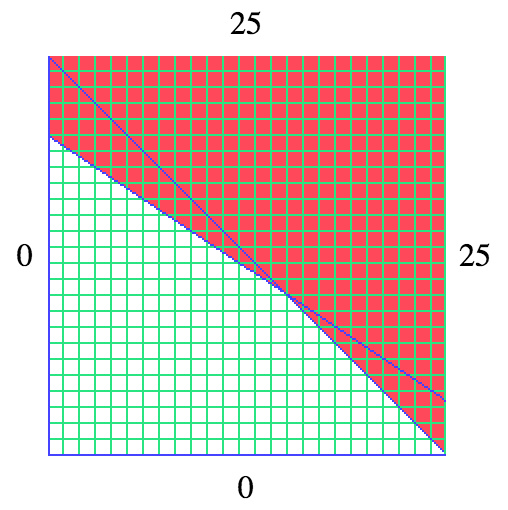
\includegraphics[width=0.5\textwidth]{example-graph.png}
    \caption{Graphical representation of the linear program example. Figure taken from \url{http://www.zweigmedia.com/}\cite{zweigmedia}}
\end{figure}

To find the optimal solution, we use the simplex method \cite{LPChvatal, LPVanderbei}.
The simplex method finds an optimal point by moving from point to point until it finds the best one.
It starts off by selecting a point in a graph.
Then it moves to a different point of the graph. On each move, it will make sure that the point yield higher
objective value. The algorithm stops when it is unable to find a point with higher objective value.
Simplex only works when the linear program has a bounded feasible region. The illustration of this algorithm is shown in figure 2.2.
For the complete explanation on the simplex method, refer to these books \cite{LPChvatal, LPVanderbei}.
\begin{figure}[!ht]
  \centering
    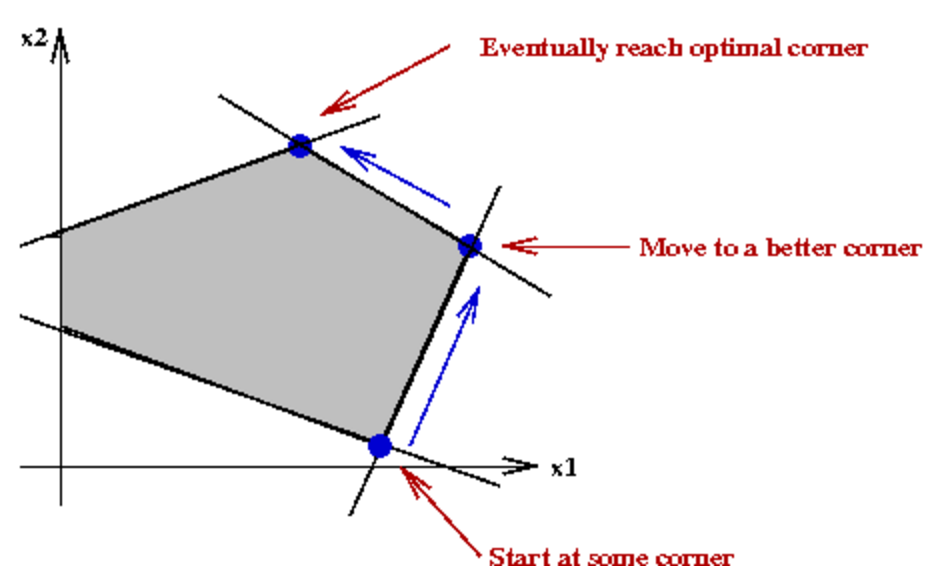
\includegraphics[width=0.8\textwidth]{simplex2.png}
    \caption{Simplex method on a linear program, taken from George Washington University \cite{seas:SM}}
    \vspace{1cm}
    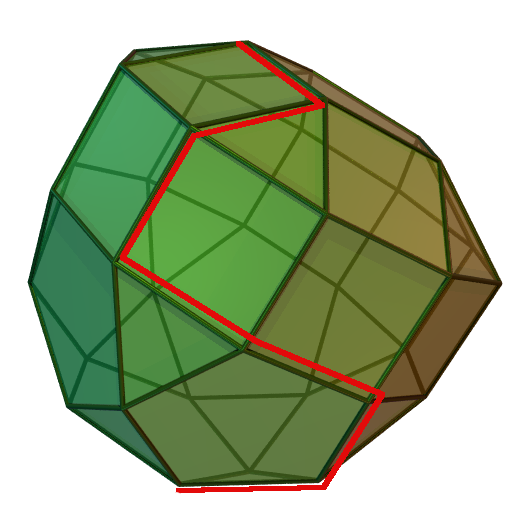
\includegraphics[width=0.5\textwidth]{simplex3d.png}
    \caption{Simplex algorithm on a 3D space, taken from Wikipedia \cite{Wiki:SPM}}
    \vspace{1cm}
\end{figure}

\section{Integer Programming}
Integer programming (IP) \cite{LPVanderbei} is LP that has an additional
integrality constraint of imposed on to its decision variables. This is useful in situations where the variables need to be
discrete, such as variables representing the number of people or boolean values.
When this constraint is added, finding an optimal solution becomes harder, as denoted by its complexity.
IP problems are in the NP Class \cite{Papadimitriou1981}, whereas LP problems are in the P class \cite{Megiddo1987}.
 IP is harder because the solution space is reduced to
the lattice points of feasible region, thereby adding more complexity in identifying the feasible solutions.
Linear programming that has both real valued and integer valued constraints on its
 decision variables is called Mixed Integer Programming (MIP) \cite{LPVanderbei}.
\begin{figure}[!ht]
  \centering
    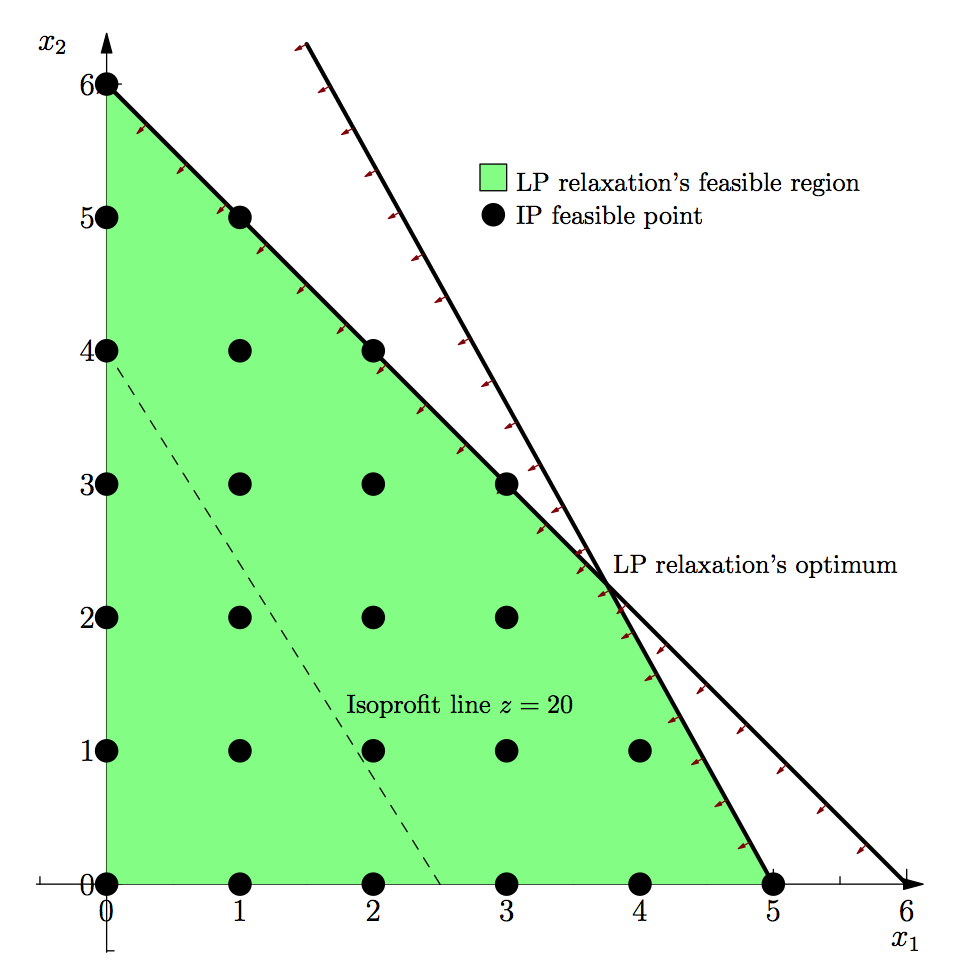
\includegraphics[width=0.7\textwidth]{ipfeasible.png}
    \caption{Feasible solutions of an integer program marked by the black dots (lattice points) bounded by the feasible region (green region), taken from
     Linear Programming: Foundations and Extensions by Robert Vanderlei \cite{Sottinen2009}}
\end{figure}

More sophisticated algorithms have been invented in order to accomodate the added complexity of IP. One of the most commonly
used algorithm that uses exact approach to finding a solution is the branch-and-bound algorithm  \cite{LPVanderbei, LPChvatal, Dastghaibifard2008}. It uses divide and
conquer approach to partition the problem into sub-problems
and then solves them recursively. LP methods such as the simplex can be used to solve the sub-problems \cite{Dastghaibifard2008}.
The 'branching' part generates a tree
that continues to expand until all valid solutions are found. The bound part compares all solutions and keeps the
most optimal one.

\section{Constraints Programming}
Unlike the programming that we have observed so far, constraints programming (CP) is a programming paradigm that is implemented
in LP solvers \cite{wiki:cp}. It is a programming paradigm that combines declarative and procedural paradigm \cite{wiki:cp, Bockmayr2003}.
The goal of CP is to find feasible solutions out of large solutions space, making it
more suitable to accomodate LP. CP focuses on the constraints and variables rather than the objective function.
In this paradigm, a constraint program may be written declaratively but should be viewed as a procedure that operates on a
solution space. Each constraints will be added to a constraint store, which limits the space that must be searched.
Constraint store uses a filtering algorithm that serves as a litmus test to determine the feasibility of a solution \cite{Bockmayr2003}.
At the end of the filtering procedure, we obtain a feasible solution.

\section{Tools}
In this project, we will be using three LP tools: Gurobi\footnote{See \url{http://gurobi.com}},
or-tools\footnote{See \url{https://developers.google.com/optimization/}} and Optaplanner\footnote{See \url{http://www.optaplanner.org}}.
We have chosen Gurobi mainly due to its performance and popularity. Or-tools and Optaplanner were chosen because
their performance have not been widely documented and they show and they show a lot of promise given their active user community
and high development activity.

Gurobi is a optimisation tool built for solving LP based problems. Its LP solver is written in C and it comes with
application programming interfaces (API) to port many different programming languages including Java, C++, Python and a few others. Gurobi allows you
to build any models for any LP problem, giving users full control to implement any algorithms or heuristics that they
prefer. It claims to be the fastest solver amongst 3 other open source solvers \cite{gurobi:solvers}, none
of which are used in this project. Gurobi is one of the most expensive commercial LP solver in the industry
and its used by many corporations such as FedEx, Netflix and Google. Academic licenses is also available for universities
and its affiliated individuals for free.

or-tools by Google is an optimisation suite for solving various optimisation problems, including VRP. It contains a constraint programming
solver, unified interface for other solvers (e.g Gurobi, GLPK, etc), implemented mostly in C++. Like Gurobi, it also comes with APIs
to support other major programming languages, albeit in less variety. This tool allows to focus on modelling the problem at hand, without worrying
too much about the algorithms and the heuristics, as they have been implemented and packaged with the solver. It is an open souce
software that is used in internally at Google that offers various advantages such as: high quality, portability and active user community.

Optaplanner is an constraint programming engine built in Java for solving optimisation problems. Unlike the other two solvers, it does not
have API to support other languages. In addition, it takes the input in the form of XML file, which are then processed by the engine. It has
predefined XML tags used to model various problems and built-in implementation of algorithms and heuristics for solving them. What Optaplanner
lacks in portability, it makes it up in usability. The XML input format allows users to define the problem rather than implementing the procedures
to solve the problem. In addition to usability, it comes with a graphical user interface (GUI) that visualise common optimisation problems, including the VRP.

\section{Graph Theory}
In this section we discuss some relevant terminologies \cite{wilson1996} from graph theory to get a better understanding of
the ideas discussed in the vehicle routing problem:
\begin{itemize}
\item A \textbf{graph} is a collection of points connected by lines in a plane. The points and lines are
more commonly refered to as \textbf{vertices} and \textbf{edges} respectively.
\item A \textbf{directed} graph is a graph whose edges goes in one direction but not the other.
\item An \textbf{undirected} graph has edges that goes in both directions.
\item A \textbf{complete} graph where all of its vertices are connected to one another.
\item A \textbf{walk} is a sequence of vertex and edges that connects one vertex to another in a graph.
\item A \textbf{path} is a walk in which no vertex appers more than once. It is also more commonly refered to as a \textbf{hamiltonian path}.
\item A \textbf{cycle} is a walk such that the first vertex corresponds with the last.
\item A \textbf{hamiltonian cycle} is hamiltonian path that also happens to be a cycle.
\end{itemize}

\section{Solution Methods and Complexity of VRP}
Solution methods come in two categories: exact approaches and heuristics. Exact approaches attempt
to find the optimal solution and will not stop until it finds one of the best \cite{neo:exact}. Some examples
include branch-and-bound \cite{LPVanderbei} and the branch-and-cut algorithm \cite{ILPCoursera}. On the other hand, heuristics approach
 attempts to solve a problem more quickly at the expense of optimality and precision. Heuristics attempts to obtain the optimal solution by incrementally improve
 the current solution \cite{Laporte1999}. We use this technique in
solving problems that may take too long to compute the exact answer or when exact algorithms failed to find any solution \cite{neo:exact}.

Lenstra et al states that all variants of VRP are NP-Hard \cite{Lenstra1981}. The implication of this is that it may
take a really long time to compute certain instances of VRP. Thus, heuristics based approach may be preferrable as opposed to
the exact one.

\section{Review}
In this chapter, we have introduced the related works and the key concepts of this project. Linear programming is a
mathematical method concerns with finding an optimal value of a function in a linear system under a set of constraints. Integer
programming is linear programming with the additional constraint where all of its decision variables are restricted to integers.
There are several algorihtms to find the optimal value of the objective function in a linear program such as simplex and branch-and-bound
algorithm. We also explained constraints programing, a programming paradigm to solve linear programs and
some background information on LP tools used in this project. We also covered some basic
concepts in graph theory that will be mentioned quite frequently throughout the project. Lastly, we discussed the
computational complexity and how it impacts the computation of VRP.

In the next chapter, we will create LP formulations and produce the requirements and the deliverables for the company involved.

% chapter 3
\chapter{Requirements and Analysis}
In this chapter, we will focus on creating the LP formulations and identifying the requirements to solve the given problem.

\section{Problem Definition}
In one busy day, the company is scheduled to make deliveries to 226 customers across the country. The deliveries are made to the customers' location by delivery vehicles. All vehicles are
expected deliver all of the customers' goods in one visit.  There are 16 of these vehicles and they are based in
one central location (depot), where the company's goods are stored. The delivery vehicles only operate on
a time window from 09:00 to 17:00. On each delivery to a customer, it takes an average of 15 minutes for the workers to successfully unload the goods.
The company wants to find the routes that yield the minimum (optimal) distance and such that all customers are visited only once. They are interested
in finding the vehicle routes that yield the minimum distance for both with and without the time windows.
The company also wants to find out if it can use less vans to make all deliveries while
keeping the total distance roughly the same (or less) as deliveries with 16 vehicles. The vehicles may serve up to 50 customers in a single tour.

We may make the following assumptions for convenience in modelling the LP formulations:
\begin{enumerate}
\item The service time for all deliveries is set to 15 minutes.
\item All delivery vehicles are homogeneous and have very large capacity (up to 50 items).
\item Customers must receive all of their goods in a single visit, so we may set all customers' demand to 1.
\item The cost function is set to the distance travelled.
\item Distance from one point to another may be calculated using the euclidian formula. We may use the haversine
formula\footnote{See \url{https://en.wikipedia.org/wiki/Haversine_formula}} to get real distance in km.
\item Traffic conditions are negligible and we assume that the roads from one point to another are straight. We make this
assumption due to lack of data.
\end{enumerate}

In addition to solving their vehicle routing problem,  the company would like to compare popular LP tools
 so that they may use the one that suits their needs. To accomplish this, we should conduct a performance analysis on the chosen LP tools
and analyse their respective features.

\section{Mathematical Formulation}
We can specifically define the problem given in the previous section with two known VRP models: capacitated
vehicle routing problem (CVRP) \cite{Daneshzand2011} and capacitated vehicle routing problem
with time windows model (CVRPTW) \cite{Daneshzand2011, Desrochers1988}, both of which has a single depot.

The CVRP model has the following input:
\begin{itemize}
\item A complete graph \(G = (V, E)\). which consists of the vertices \(V\) and the edges \(E\).
\item The variable \(n\), which represent the total number of customers and the depot.
\item The variable \(K\), which represent the total number of vehicles available. This will dictate the number of routes
generated in the model, with each vehicle having its own route.
\item A vertex set \(V\), numbered from 1 to \(n\) and vertex 1 is the depot.
\item A set of edges for \(V\).
\item The cost function \(c_{ij}\) that outputs the distance travelled from vertex i to j, where \(i,j \in V\).
\item The path function \(x_{ij}\) that outputs 1 if the path i to j is included in the current journey and 0 otherwise.
\item The capacity function \(r(S)\) that outputs the number capacity needed to serve a set of customers \(S\).
\end{itemize}

Given the input above, we can create a single depot capacitated vehicle routing problem below:

\vspace{0.5cm}

\begin{equation}
    \begin{array}{ll@{}ll}
        \text{Minimize} & \displaystyle\sum\limits_{i \in V}\sum\limits_{j \in V} c_{ij}&x_{ij} &\\
    \end{array}
\end{equation}
\begin{equation}
    \begin{array}{ll@{}ll}
        \text{Subject to}&\displaystyle\sum\limits_{i \in V}   &x_{ij} = 1,  &\forall j \in V \setminus \{1\}\\
    \end{array}
\end{equation}
\begin{equation}
    \begin{array}{ll@{}ll}
        & \displaystyle\sum\limits_{j \in V}   &x_{ij} = 1,  &\forall i \in V \setminus \{1\}\\
    \end{array}
\end{equation}
\begin{equation}
    \begin{array}{ll@{}ll}
        & \displaystyle\sum\limits_{i \in V}   &x_{1i} = K\\
    \end{array}
\end{equation}
\begin{equation}
    \begin{array}{ll@{}ll}
        & \displaystyle\sum\limits_{i \in V}   &x_{i1} = K\\
    \end{array}
\end{equation}
\begin{equation}
    \begin{array}{ll@{}ll@{}ll}
        & \displaystyle\sum\limits_{i \in S}\sum\limits_{i \in S}  &x_{ij} \leq |S| - r(S), &\forall S \subseteq V/ \{1\} , S \neq \oldemptyset \\
    \end{array}
\end{equation}
\begin{equation}
    \begin{array}{ll@{}ll@{}ll}
        & x_{ij} = \{0,1\}\\
    \end{array}
\end{equation}

\vspace{1cm}

Equations (3.2) and (3.3) are constraints to ensure that all cities are visited only once, excluding the depot. Constraints (3.4) and (3.5)
impose the vehicles coming in must be equal to the vehicles coming out of the depot. Constraint (3.6) is the Subtour
Elimination Constraint (SEC) to ensure that each route is a hamiltonian cycle. This is to ensure that routes are optimal
 and accurately represent the situation in real life. Subtours are
cycles that exists within a set of vertices that partition the set into two or more components. Figures
3.2 and 3.3 illustrates the difference between a graph with subtours and a graph with a hamiltonian cycle.
\vspace{0.5cm}
\begin{figure}[!ht]
  \centering
    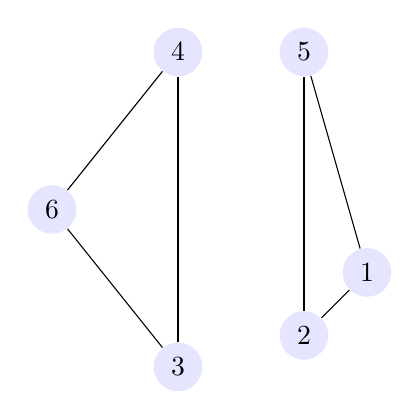
\begin{tikzpicture}
          [scale=.4,every node/.style={circle,fill=blue!10}]
          \node (n6) at (1,10) {6};
          \node (n4) at (5,15)  {4};
          \node (n5) at (9,15)  {5};
          \node (n1) at (11,8) {1};
          \node (n2) at (9,6)  {2};
          \node (n3) at (5,5)  {3};

          \foreach \from/\to in {n6/n4,n5/n1,n1/n2,n2/n5,n3/n4,n6/n3}
            \draw (\from) -- (\to);

        \end{tikzpicture}

      \caption{A graph with subtours}
      \label{fig:subtour}
\end{figure}

\begin{figure}[!ht]
  \centering
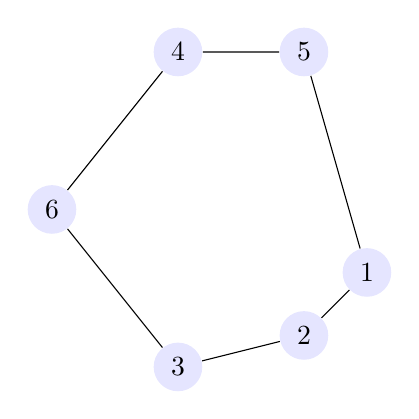
\begin{tikzpicture}
          [scale=.4,every node/.style={circle,fill=blue!10}]
          \node (n6) at (1,10) {6};
          \node (n4) at (5,15)  {4};
          \node (n5) at (9,15)  {5};
          \node (n1) at (11,8) {1};
          \node (n2) at (9,6)  {2};
          \node (n3) at (5,5)  {3};

          \foreach \from/\to in {n6/n4,n5/n1,n4/n5,n1/n2,n6/n3,n3/n2}
            \draw (\from) -- (\to);

        \end{tikzpicture}
      \caption{A graph with a hamiltonian cycle}
      \label{fig:hamiltoniancycle}
\end{figure}


There are two common formulations to eliminate subtours: the MTZ formulation by Miller \cite{Miller1960} and
the Subtour Formulation \cite{Lawler1985, Pataki2003}. Pataki \cite{Pataki2000} states that Subtour Elimination is the efficient formulation to reach optimal solution, whereas
the MTZ Formulation is highly inefficient despite its elegance. We formulate constraint (3.6) by combining capacity cut constraint (CCC), a constraint to ensure
that the vehicles meet the demands of all customers in a tour, with the Subtour Formulation to get the SEC for VRP \cite{Daneshzand2011}.

In order to model CVRPTW, we need to introduce a new set of input related to time window constraints:
\begin{itemize}
\item Variable \(D_{i}\) that represents the departure time to customer \(i\).
\item Time function \(t_{ij}\) that outputs the time taken to travel to customer \(i\) to \(j\).
\item Variable \(e_{i}\) that represents the earliest time for visiting customer \(i\).
\item Variable \(l_{i}\) that represents the latest time for visiting customer \(i\).
\item Variable \(y_{i}\) that represents the remaining capacity of the vehicle when visiting customer \(i\).
\item Variable \(q_{i}\) that represents the demand of customer \(i\).
\item Variable \(Q\) that represent the capacity of the vehicle \(i\).
\end{itemize}

Putting it together, we have the complete CVRPTW model below:

\vspace{0.5cm}

\begin{equation}
    \begin{array}{ll@{}ll}
        \text{Minimize} & \displaystyle\sum\limits_{i \in V}\sum\limits_{j \in V} c_{ij}&x_{ij} &\\
    \end{array}
\end{equation}
\begin{equation}
    \begin{array}{ll@{}ll}
        \text{Subject to}&\displaystyle\sum\limits_{i \in V}   &x_{ij} = 1,  &\forall j \in V \setminus \{1\}\\
    \end{array}
\end{equation}
\begin{equation}
    \begin{array}{ll@{}ll}
        & \displaystyle\sum\limits_{j \in V}   &x_{ij} = 1,  &\forall i \in V \setminus \{1\}\\
    \end{array}
\end{equation}
\begin{equation}
    \begin{array}{ll@{}ll}
        & \displaystyle\sum\limits_{i \in V}   &x_{1i} = K\\
    \end{array}
\end{equation}
\begin{equation}
    \begin{array}{ll@{}ll}
        & \displaystyle\sum\limits_{i \in V}   &x_{i1} = K\\
    \end{array}
\end{equation}
\begin{equation}
    \begin{array}{ll@{}ll@{}ll}
        & \displaystyle\sum\limits_{i \in S}\sum\limits_{i \in S}  &x_{ij} \leq |S| - r(S), &\forall S \subseteq V/ \{1\} , S \neq \oldemptyset \\
    \end{array}
\end{equation}
\begin{equation}
    \begin{array}{ll@{}ll@{}ll}
        & x_{ij} = \{0,1\}\\
    \end{array}
\end{equation}
\begin{equation}
    \begin{array}{ll@{}ll@{}ll}
        & x_{ij} = 1 \implies D_{i} + t_{ij} \leq D_{j}, \forall i, j \in V / \{1\}
    \end{array}
\end{equation}
\begin{equation}
    \begin{array}{ll@{}ll@{}ll}
        & e_{i} \leq D_{i} \leq l_{i}, \forall i \in V / \{1\}
    \end{array}
\end{equation}
\begin{equation}
    \begin{array}{ll@{}ll@{}ll}
        & x_{ij} = 1 \implies y_{i} + q_{i} \leq y_{j}, \forall i, j \in V / \{1\}
    \end{array}
\end{equation}
\begin{equation}
    \begin{array}{ll@{}ll@{}ll}
        & 0 \leq y_{i} \leq Q, \forall i \in V / \{1\}
    \end{array}
\end{equation}

\vspace{1cm}

Constraint (3.15) ensures that given a chosen path from vertex i to j, the departure time of j does not exceed the
departure time at vertex i plus the time taken to travel from vertex i to j. Constraints (3.17) and (3.18) are the
demand and capacity constraints to ensure that the capacity does not exceed the demand at any point in the given route.

\section{Requirements}
Based on the problem and formulations in the previous section,
we have identified a list of requirements needed to solve the stated problem.
The requirements are a list of of criteria to ensure that our analysis is done correctly and produce the desired results.
MoSCoW framework is used to denote their respective priority. The table below contains the requirements for this project:
\vspace{0.5cm}
\begin{table}[!ht]
\centering
\begin{tabular}{|l|p{8cm}|l|}
\hline
ID & Requirement                                                                                                                                                     & Priority    \\ \hline
R1  & CVRP and CVRPTW models must fulfill the subtour elimination constraints that will ensure that all routes are hamiltonian cycles                                                                                                   & Must Have   \\ \hline
R2  & CVRP and CVRPTW models must fulfill the constraints where the number of vehicles entering and leaving the depot is the same                                                                                                       & Must Have   \\ \hline
R3  & CVRP and CVRPTW models must fulfill the constraint where the vehicle capacity must not exceed the total demand of customers on a given route                                                                                               & Must Have   \\ \hline
R4  & CVRPTW models  must fulfill time window constraints                                                                                               & Must Have   \\ \hline
R5  & CVRP models chosen to solve the given VRP problem must perform well on benchmark and test datasets                                                                & Must Have   \\ \hline
R6  & LP models must be able to produce the total distance of the routes                                                                                              & Must Have   \\ \hline
R7  & LP models Should be able to produce the optimal routes                                                                                                          & Should Have \\ \hline
R8  & We must be able to compare and contrast the performance and features of LP tools                                                                                & Should Have \\ \hline
R9  & The euclidian distance given in the solution should be able to be converted to kilometers                                                                       & Could Have  \\ \hline
R10 & LP tools could visualise the vehicle routes on a map/graph                                                                                                      & Could Have  \\ \hline
\end{tabular}
\caption{Requirements table}
\label{requirements-table}
\end{table}

\section{Review}
In this chapter, we have defined the problem and transformed it into two VRP formulations: CVRP and CVRPTW. VRP is problem
that concerns with finding the minimum total distance of routes for fleet of vehicles to satisfy a set of customers. CVRP is VRP
where the vehicles has maximum capacity to which it can serve customers. CVRPTW is CVRP with additional constraint that
the vehicles operate on a time window. In addition, we have defined the requirements for the stated problem listed in table 3.1.

In the next chapter, we shall discuss the how the the LP formulations are created into models using different LP tools.

% chapter 4
\chapter{Implementation}

This chapter contains the bulk of the analysis of the VRP problem. In this chapter We will discus the implementation and testing of the model
using the chosen tools.

\section{Tools}
In this project, we will be using LP tools: Gurobi, Google Optimization Tools, Optaplanner to solve the problem
defined in the previus chapter. These tools have their own unique APIs and input format. Each of them
have different implementation of the LP solver that causes them to produce different results given the same input,
as we shall see in the next chapter.

Gurobi is a optimisation tool built for solving LP based problems. Its LP solver is written in C and it comes with
APIs to port many different programming languages including Java, C++, Python and a few others. Gurobi allows you
to build any models for any LP problem, giving users full control to implement any algorithms or heuristics that they
prefer. It claims to be the fastest solver amongst 3 other open source solvers\footnote{refer to
this link}, none of which are used in this project. Gurobi is one of the most expensive commercial LP solver in the industry
and its used by many corporations such as FedEx, Netflix and Google. Academic licenses is also available for universities
and its affiliated individuals for free.

or-tools by Google is an optimisation suite for solving various optimisation problems, including VRP. It contains a constraint programming
solver, unified interface for other solvers (e.g Gurobi, GLPK, CPLEX, etc), implemented mostly in C++. Like Gurobi, it also comes with APIs
to support other major programming languages, albeit less variety. This tool allows to focus on modelling the problem at hand, without worrying
too much about the algorithms and the heuristics, as they have been implemented and packaged with the solver. It is an open souce
software that is used in internally at Google that offers various advantages such as: high quality, portability, has active user community.

Optaplanner is an constraint programming engine built in Java for solving optimisation problems. Unlike the other two solvers, it does not
have API to support other languages. In addition, it takes the input in the form of XML file, which are then processed by the engine. It has
predefined XML tags used to model various problems and built-in implementation of algorithms and heuristics for solving them. What Optaplanner
lacks in portability, it makes it up in usability. The XML input format allows users to define the problem rather than implementing the procedures
to solve the problem. In addition to usability, it comes with a nice GUI that visualise common optimisation, including the VRP.

These tools are run on the same hardware. The processor of this hardware is 2.8GHz dual-core Intel i5. It has
8GB 1600 MHz DDR3 memory and is running OSX version 10.9.5.

\section{Datasets}
We have prepared 3 datasets for this project. The first one is a benchmark dataset with known solution to test the tools
if they can find the optimal solution in a small instance. The next dataset is used to compare the compare the performance
of the tools under a time limit. The last datasets are the dataset of the actual problem given by the company. All datasets
share the same schema: Node number, Latitude and Longitude.

The details of the 3 datasets are tabulated in the table below:
\begin{table}[!ht]
    \begin{center}
        \begin{tabular}{ | l | l | p{10.5cm} |}
        \hline
        Name & Size  & Description \\ \hline
        CVRP-9 & 9 nodes  & This is benchmark dataset that is used to build a simple CVRP model to test
        if the LP tools can produce an optimal solution that are close to the known solution under a small load. The vertices in the datasets
        are arranged in such a way that the optimal routes are obvious and can be obtained without calculation.\\ \hline
        CVRP-60 & 60 nodes & This is a dataset that is used to model a CVRP model that is used to compare the performance of tools
        under a time limit of 5 minutes. We take the results generated and compare their optimality.\\ \hline
        CVRP-227 & 227 nodes & This dataset is the actual problem dataset from the company. It is used to model both CVRP and CVRPTW models
        in this project. This dataset can be used to model CVRPTW model even without time windows data because the time window variables are uniform across
        all customers. One of the main objective of this project to collect the optimal distance and its respective routes.\\
        \hline
        \end{tabular}
        \caption{Datasets description}
        \label{table:dataset_description}
    \end{center}
\end{table}

\section{Model Parameters}
The model parameters are variables that is For CVRP-9 and CVRP-60, the parameters are similar
Sets, Parameters and Variables
Capacitated Vehicle Routing Problem Model
Capacitated Vehicle Routing Problem with Time Window Model

\section{Model Implementations}
Talk about the implementation, create model with both python script and the file (Gurobi and OR tools), or just
input file (Optaplanner)


% chapter 5
\chapter{Results and Discussions}
In this chapter we will discuss the results from the analysis of benchmark datasets and the problem dataset, followed
by the discussions on the results. Finally, we give recommendation to the company based on the requirements stipulated
in chapter 3.

\section{Results}
Table 5.1 shows the result of the analysis of various benchmark datasets using Gurobi, or-tools and optaplanner. There is
a time limit imposed on each analysis. For gurobi and optaplanner, the model runs for approximately\footnote{need to account for the reaction
time of human} the full duration of time limit and whatever solution is retrieved at the end of it is recorded. For optaplanner, the tabulated
time is taken the moment its tabulated solution does not change. All solution stated is in terms of the total euclidian distance
of all routes combined.
\begin{table}[!ht]
\caption{results}
\label{table:results}
\begin{center}
\begin{tabular}{|l|l|l|l|l|l|l|}
\hline
\multirow{2}{*}{Model /\ Solver}                                                         & \multicolumn{2}{l|}{Gurobi}                              & \multicolumn{2}{l|}{or-tools}                      & \multicolumn{2}{l|}{Optaplanner}                       \\ \cline{2-7}
                                                                                         & Time                           & Solution                & Time                     & Solution                & Time                     & Solution                \\ \hline
\multirow{2}{*}{\begin{tabular}[c]{@{}l@{}}A-n32-k5\\ Best Solution: 784\end{tabular}}  & \multirow{2}{*}{leq 1s}        & \multirow{2}{*}{763.9}  & \multirow{2}{*}{< 1s} & \multirow{2}{*}{870.9}  & \multirow{2}{*}{11s}  & \multirow{2}{*}{787.1}  \\
                                                                                         &                                &                         &                          &                         &                              &                         \\ \hline
\multirow{2}{*}{\begin{tabular}[c]{@{}l@{}}A-n44-k6\\ Best Solution: 937\end{tabular}}   & \multirow{2}{*}{5 mins} & \multirow{2}{*}{849}    & \multirow{2}{*}{< 1s} & \multirow{2}{*}{1013.8} & \multirow{2}{*}{37s}  & \multirow{2}{*}{938.8}  \\
                                                                                         &                                &                         &                          &                         &                              &                         \\ \hline
\multirow{2}{*}{\begin{tabular}[c]{@{}l@{}}A-n53-k7\\ Best Solution: 1010\end{tabular}}  & \multirow{2}{*}{5 mins} & \multirow{2}{*}{925.9}  & \multirow{2}{*}{< 1s} & \multirow{2}{*}{1119.2} & \multirow{2}{*}{1:06} & \multirow{2}{*}{1057.3} \\
                                                                                         &                                &                         &                          &                         &                              &                         \\ \hline
\multirow{2}{*}{\begin{tabular}[c]{@{}l@{}}A-n65-k9\\ Best Solution: 1174\end{tabular}}  & \multirow{2}{*}{5 mins} & \multirow{2}{*}{1027}   & \multirow{2}{*}{< 1s} & \multirow{2}{*}{1284}   & \multirow{2}{*}{1:24} & \multirow{2}{*}{1187}   \\
                                                                                         &                                &                         &                          &                         &                              &                         \\ \hline
\multirow{2}{*}{\begin{tabular}[c]{@{}l@{}}A-n80-k10\\ Best Solution: 1763\end{tabular}} & \multirow{2}{*}{5 mins} & \multirow{2}{*}{1484.1} & \multirow{2}{*}{< 1s} & \multirow{2}{*}{1948.2} & \multirow{2}{*}{2:00} & \multirow{2}{*}{1797.6} \\
                                                                                         &                                &                         &                          &                         &                              &                         \\ \hline
\multirow{2}{*}{\begin{tabular}[c]{@{}l@{}}T-VRP-9\\ Best Solution: N.A\end{tabular}}    & \multirow{2}{*}{5 mins} & \multirow{2}{*}{34.6}   & \multirow{2}{*}{< 1s} & \multirow{2}{*}{34.7}   & \multirow{2}{*}{leq 1s}      & \multirow{2}{*}{31.5}   \\
                                                                                         &                                &                         &                          &                         &                              &                         \\ \hline
\multirow{2}{*}{\begin{tabular}[c]{@{}l@{}}P-VRP-60\\ Best Solution: N.A\end{tabular}}   & \multirow{2}{*}{5 mins} & \multirow{2}{*}{3.1}    & \multirow{2}{*}{< 1s} & \multirow{2}{*}{10.5}   & \multirow{2}{*}{1:04} & \multirow{2}{*}{2.9}    \\
                                                                                         &                                &                         &                          &                         &                              &                         \\ \hline
\end{tabular}
\end{center}
\end{table}

Based on the results above other considerations, we have decided to use oplaplanner to analyse the VRP problem.
We have analysed the CVRP and CVRPTW models based on the formulation in chapter 3 and tabulated the results in
table 5.2 below:
\begin{table}[!ht]
\centering
\begin{tabular}{|l|l|l|l|}
\hline
Model  & Time Window & Solution & Actual Distance \\ \hline
CVRP   & No          & 10.27   & 798.57\\ \hline
CVRPTW & Yes         & 10.49   & 828.95\\ \hline
\end{tabular}
\caption{Results of analysis of VRP problem}
\label{my-label}
\end{table}
Both models have the following parameters:
\begin{itemize}
\item P-VRP-227 dataset
\item Time limit of 5 mins
\item has 8 vehicles, each of which is capable of delivering 29 items.
\item 226 customers
\end{itemize}

For CVRPTW model, the earliest and latest time for delivery for all customers is set to 09:00 and 17:00 respectively. The
service time is set to 15 minutes.

These are the routes of the two models are tabulated in figure 5.3 and 5.4. The numbers represent the node number and
they are arranged in order of which customers get visited first.
\begin{table}[!ht]
\centering
\caption{Routes}
\label{my-label}
\begin{tabular}{|l|l|}
\hline
\multicolumn{2}{|l|}{CVRP Model}                                                                      \\ \hline
Vehicle No         & Order of visit                                                                         \\ \hline
\multirow{2}{*}{1} & \multirow{2}{*}{\begin{tabular}[c]{@{}l@{}}48, 57, 75, 70, 102, 87, 79, 96, 97, 91, 144, 126, 146, 145,\\ 163, 188, 182, 187, 171, 189, 143, 62, 156, 167, 134, 76, 45, 29\end{tabular}} \\
                   &                                                                                  \\ \hline
\multirow{2}{*}{2} & \multirow{2}{*}{\begin{tabular}[c]{@{}l@{}}24, 54, 68, 67, 85, 80, 110, 152, 180, 191, 193, 196, 181, 147,\\ 175, 113, 108, 83, 78, 130, 136, 154, 105, 73, 53, 23, 44, 41, 22\end{tabular}}  \\
                   &                                                                                  \\ \hline
\multirow{2}{*}{3} & \multirow{2}{*}{\begin{tabular}[c]{@{}l@{}}25, 40, 127, 107, 141, 199, 202, 209, 192, 213, 217, 222, 201,\\ 210, 208, 204, 206, 214, 207, 195, 205, 112, 92, 88, 104, 93\end{tabular}} \\
                   &                                                                                  \\ \hline
\multirow{2}{*}{4} & \multirow{2}{*}{\begin{tabular}[c]{@{}l@{}}32, 47, 59, 21, 26, 43, 31, 114, 98, 178, 172, 176, 161, 165,\\ 185, 216, 225, 218, 226, 227, 224, 220, 223, 215, 184, 103, 74, 63, 37\end{tabular}}  \\
                   &                                                                                  \\ \hline
\multirow{2}{*}{5} & \multirow{2}{*}{\begin{tabular}[c]{@{}l@{}}36, 60, 56, 128, 153, 140, 133, 166, 139, 162, 194, 183, 168,\\ 173, 155, 135, 115, 95, 72, 77, 94, 61, 99, 124, 86, 109, 123\end{tabular}}  \\
                   &                                                                                  \\ \hline
\multirow{2}{*}{6} & \multirow{2}{*}{\begin{tabular}[c]{@{}l@{}}71, 33, 69, 46, 42, 82, 65, 131, 132, 164, 169, 150, 177, 190,\\ 125, 116, 66, 118, 119, 106, 101, 138, 84, 90, 120, 142, 121, 111, 52\end{tabular}}  \\
                   &                                                                                  \\ \hline
\multirow{2}{*}{7} & \multirow{2}{*}{\begin{tabular}[c]{@{}l@{}}17, 20, 30, 19, 15, 13, 14, 35, 34, 38, 39, 28, 64, 58, 49, 51,\\ 55, 16, 18, 12, 50, 9, 10, 11, 7, 8, 2, 4, 5\end{tabular}}  \\
                   &                                                                                  \\ \hline
\multirow{2}{*}{8} & \multirow{2}{*}{\begin{tabular}[c]{@{}l@{}}3, 6, 89, 151, 129, 157, 122, 137, 159, 158, 117, 174, 198, 186,\\ 212, 211, 221, 219, 200, 203, 197, 179, 170, 149, 160, 148, 100, 81, 27\end{tabular}}  \\
                   &                                                                                  \\ \hline
\end{tabular}
\end{table}

\begin{table}[!ht]
\centering
\caption{Routes}
\label{my-label}
\begin{tabular}{|l|l|}
\hline
\multicolumn{2}{|l|}{CVRPTW Model}                                                                      \\ \hline
Vehicle No         & Order of visit                                                                           \\ \hline
\multirow{2}{*}{1} & \multirow{2}{*}{\begin{tabular}[c]{@{}l@{}}3, 151, 157, 85, 129, 122, 137, 159, 117, 158, 174, 136, 108, 95,\\ 113, 198, 179, 197, 203, 212, 211, 221, 219, 200, 89, 8, 7, 2\end{tabular}} \\
                   &                                                                                  \\ \hline
\multirow{2}{*}{2} & \multirow{2}{*}{\begin{tabular}[c]{@{}l@{}}24, 40, 41, 27, 81, 148, 110, 78, 72, 83, 80, 77, 115, 149, 186,\\ 191, 181, 196, 193, 152, 133, 61, 140, 94, 124, 99, 54, 44\end{tabular}}  \\
                   &                                                                                  \\ \hline
\multirow{2}{*}{3} & \multirow{2}{*}{\begin{tabular}[c]{@{}l@{}}25, 60, 56, 86, 100, 135, 166, 139, 155, 194, 162, 183, 173, 168,\\ 170, 160, 180, 175, 147, 130, 154, 105, 73, 68, 67, 53, 23, 36, 22\end{tabular}} \\
                   &                                                                                  \\ \hline
\multirow{2}{*}{4} & \multirow{2}{*}{\begin{tabular}[c]{@{}l@{}}55, 37, 63, 31, 93, 123, 109, 127, 141, 128, 153, 107, 199, 202,\\ 209, 192, 201, 210, 222, 217, 213, 204, 208, 205, 185, 172, 91, 104, 48\end{tabular}}  \\
                   &                                                                                  \\ \hline
\multirow{2}{*}{5} & \multirow{2}{*}{\begin{tabular}[c]{@{}l@{}}75, 102, 103, 145, 176, 184, 215, 220, 223, 224, 227, 226, 225,\\ 216, 218, 195, 214, 207, 206, 178, 161, 165, 112, 98, 92, 88, 114, 43, 26\end{tabular}}  \\
                   &                                                                                  \\ \hline
\multirow{2}{*}{6} & \multirow{2}{*}{\begin{tabular}[c]{@{}l@{}}52, 111, 118, 119, 106, 101, 142, 121, 120, 90, 84, 190, 177,\\ 116, 125, 164, 169, 150, 134, 132, 131, 82, 65, 76, 46, 69, 70, 57\end{tabular}}  \\
                   &                                                                                  \\ \hline
\multirow{2}{*}{7} & \multirow{2}{*}{\begin{tabular}[c]{@{}l@{}}32, 47, 59, 21, 87, 97, 126, 163, 146, 144, 188, 182, 187, 96,\\ 79, 74, 143, 62, 156, 189, 171, 167, 45, 42, 29, 33, 71\end{tabular}}  \\
                   &                                                                                  \\ \hline
\multirow{2}{*}{8} & \multirow{2}{*}{\begin{tabular}[c]{@{}l@{}}19, 20, 30, 17, 14, 13, 15, 35, 34, 38, 28, 39, 64, 138, 66, 58,\\ 49, 51, 4, 5, 6, 11, 16, 10, 9, 50, 12, 18\end{tabular}}  \\
                   &                                                                                  \\ \hline
\end{tabular}
\end{table}

Visualisation of CVRP and CVRPTW model:

\begin{figure}[!ht]
  \centering
    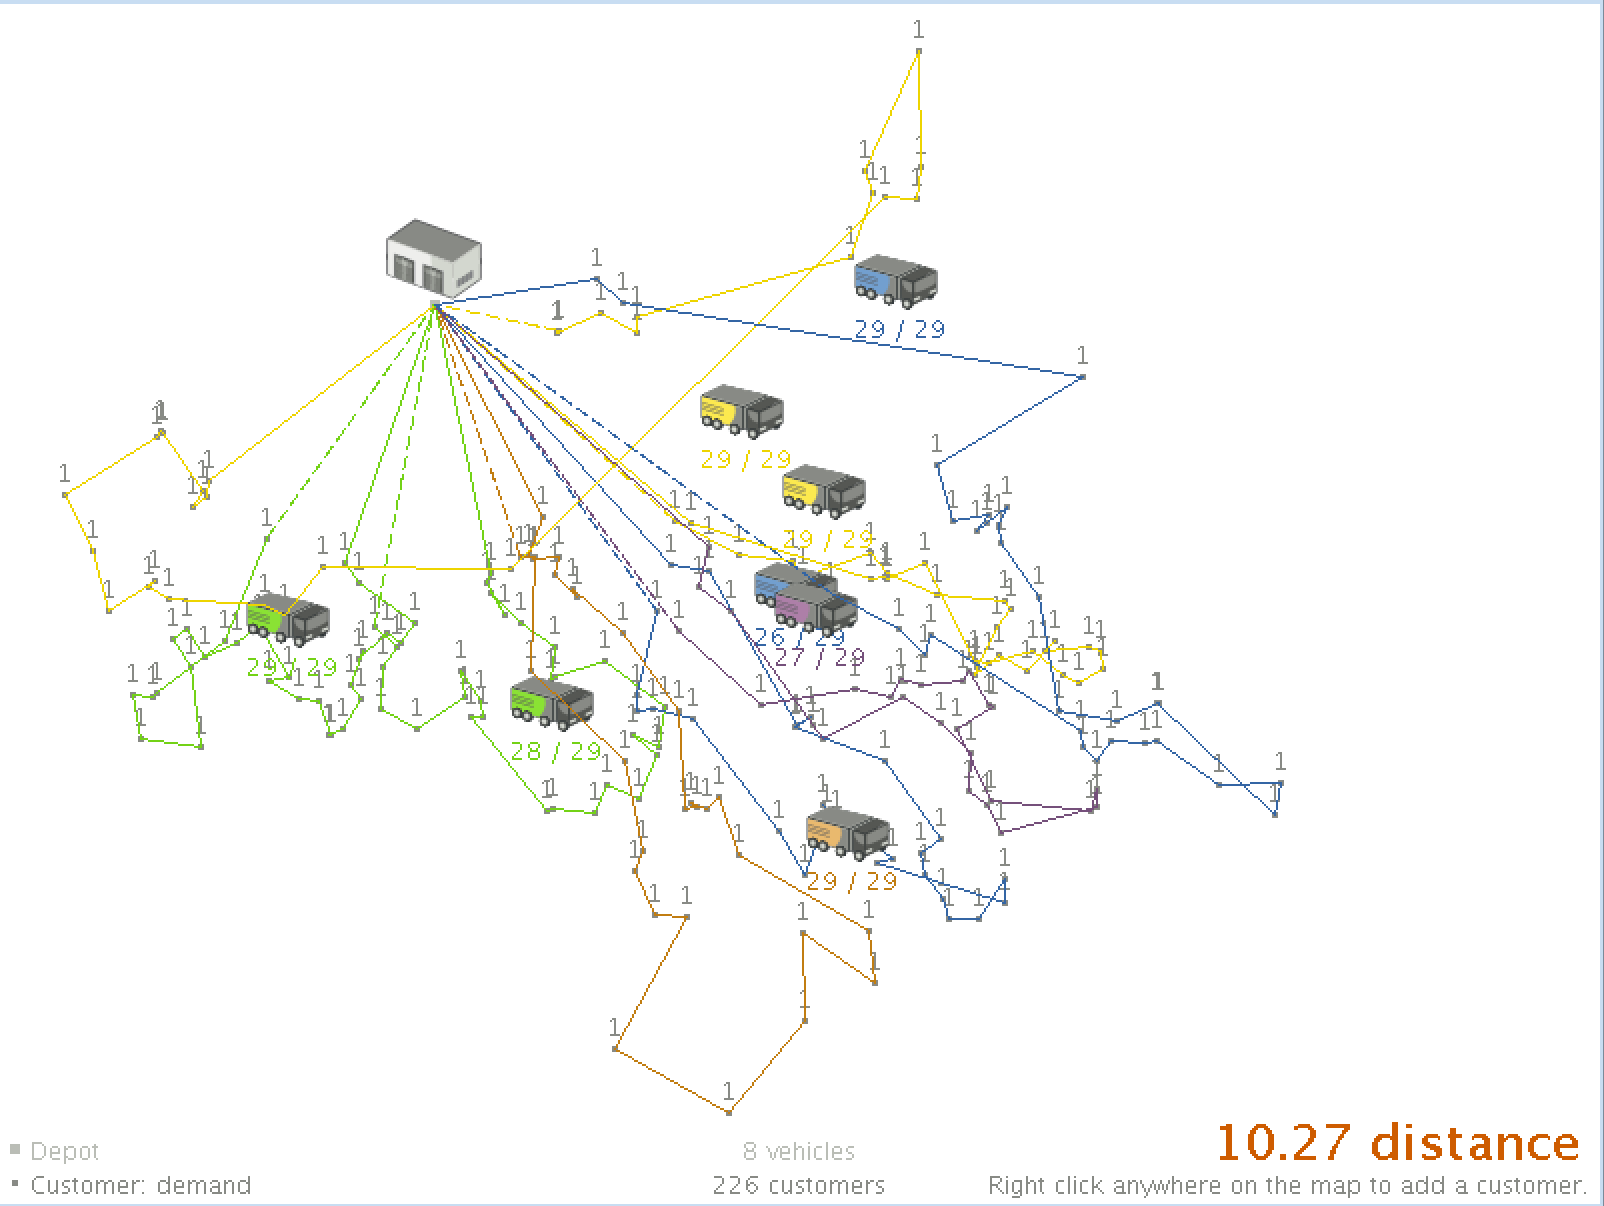
\includegraphics[width=1\textwidth]{227-cvrp.png}
    \caption{Visualisation of CVRP Model}
\end{figure}

\begin{figure}[!ht]
  \centering
    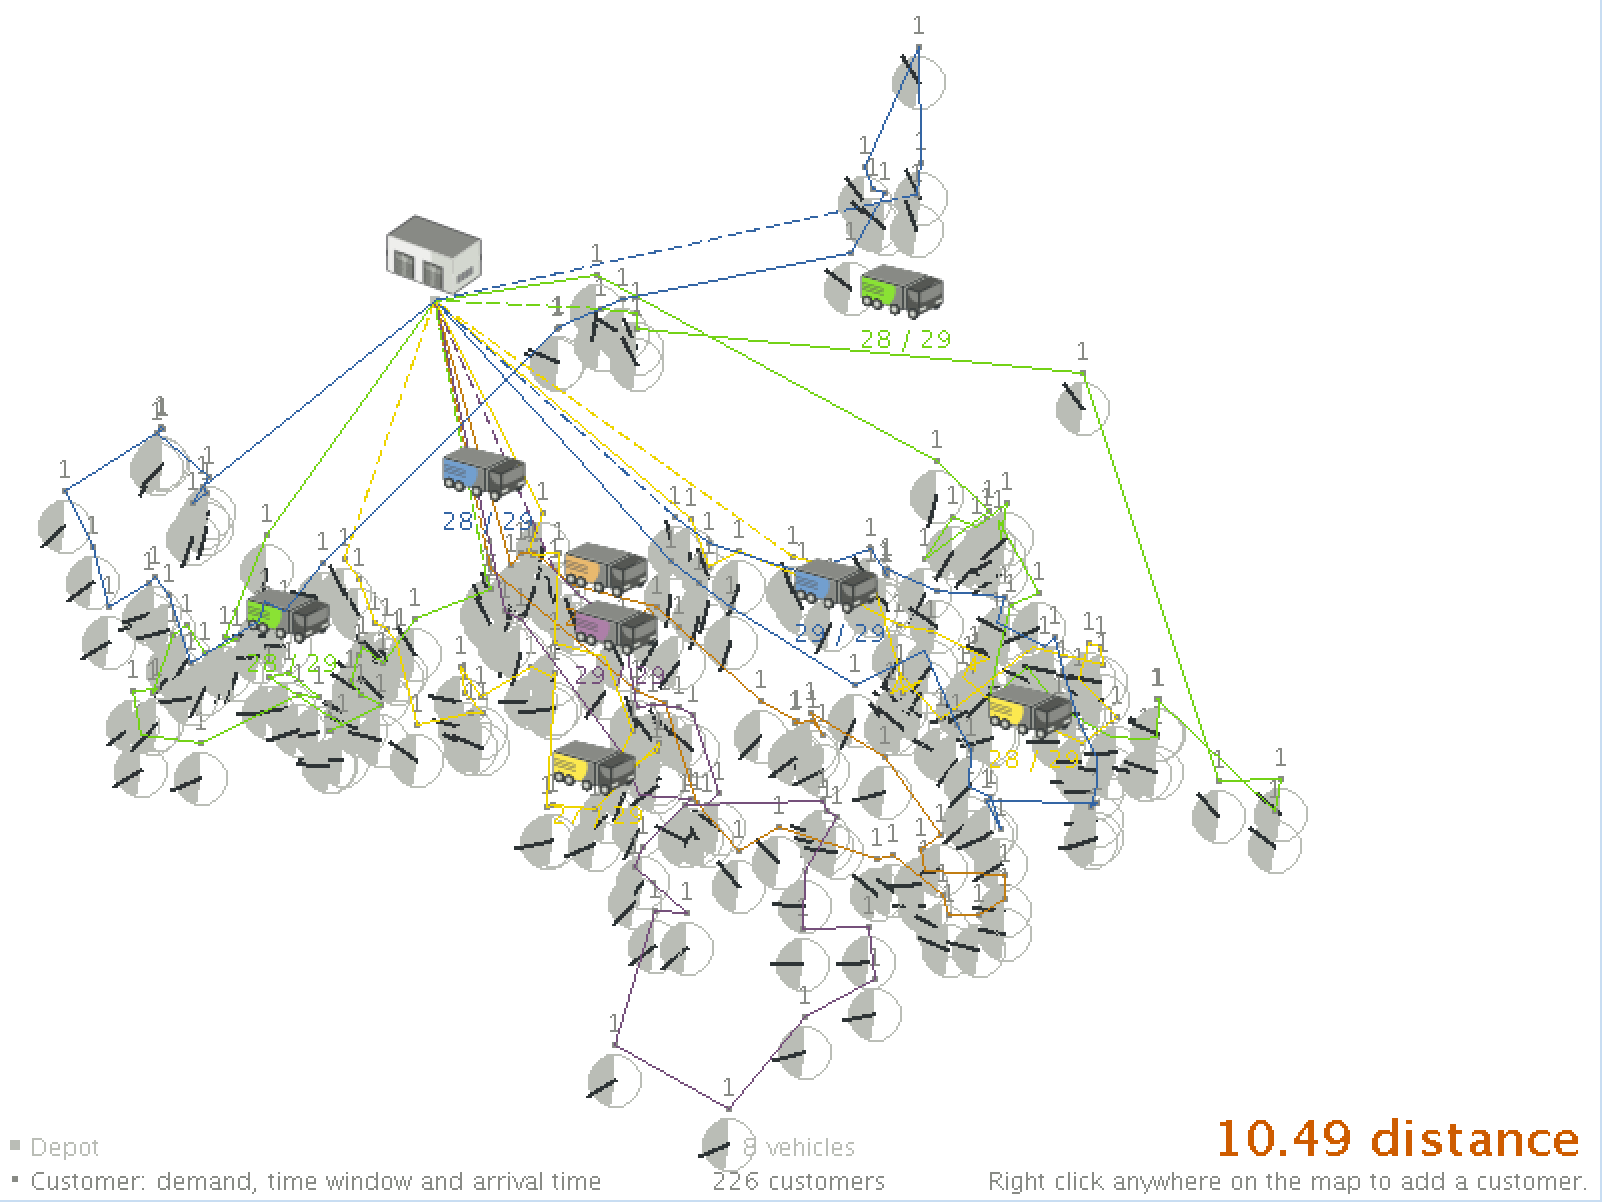
\includegraphics[width=1\textwidth]{227-cvrptw.png}
    \caption{Visualisation of CVRPTW Model}
\end{figure}

\section{Discussions}
\begin{enumerate}
\item Performance analysis of LP tools. Overall, Gurobi outperforms or-tools and optaplanner on all the models with
benchmark datasets. The optimal results obtained are even better than the known solution. We assume that the model is
correct, given the fact that it performs well on the test instance.
Or-tools underperforms on all cases using cheapest arc heuristics. Using different heuristics does not
improve the results and may take too long to terminate. Optaplanner gives a solution that is close to the best known result
 and gives the best performance for P-VRP-60, which indicates that it may be more suitable to use on a given problem.
 here are some pros and cons of using the tools, we only comment on the its application in VRP based problems.

\item Why Optaplanner? There are a few reasons to choose optaplanner. Firstly, it yields the best solution for the instance
of CVRP based on the given problem. It is easy to create a model and free: these two criteria is important, considering that
the requests made by the company.

\item talk about parameter estimation. We estimate the parameters such as the number of vehicles and its maximum capacity by trial
and error. There are 227 nodes, so the minimum number of edges to traverse all the edges once is 227. So, we get the combination of vehicles
and capacity by multiplying them such that the product is slightly greater than 227. In our analysis, using 8 vehicles and with 29 capacity
yields the best result.

\item How accurate is the model compared to the real life scenario?
 We are using air distance, which does not accurately present
the roads in traffic as they are never straight. This may undermine the quality of the solution
 In addition, we need to use the haversine function on the routes to get the distance covered in km. However, this solution
 would definitely be efficient enough to save the company money when utilised, as opposed to using manual route planning.

\item Advantages and Disadvantages of using each tool and suggest which tool to use given user profile.
\end{enumerate}

\begin{table}[!ht]
\centering
\caption{My caption}
\label{my-label}
\begin{tabular}{|l|p{0.2\textwidth}|p{0.2\textwidth}|p{0.3\textwidth}|}
\hline
Tools       & Advantages & Disadvantages & Comments \\ \hline
Gurobi      & High performance, good APIs to interface other languages, easy to install, and more control on model implementation.
            & Costs money when used for business and relatively hard to use
            & This tool is suitable for companies with sizeable budget on the data analysis department and more experienced OR analysts. \\ \hline
Or-tools    & good APIs to interface popular languages,free, open source  &  Relatively poor performance and hard to install  & This tool is suitable for hobbysts and experienced programmers who would like to look at examples and optimise their own solver\\ \hline
Optaplanner &  Good performance, comes with GUI, free, open source, easy to model formulation &     only support Java     & Good tool for learning how to solve planning problems. Can also be used at enterprise level...  \\ \hline
\end{tabular}
\end{table}

\section{Review}
Review this chapter... balh dih blah lorem ipsum dolor amet


% chapter 6
\chapter{Conclusions and Future Work}
In here I shall conclude a few things: we've started off with a primer on linear programming and discussed its state
 of the art. Obtained the optimal routes that yields the minimum distance and the number of vehicles to use. Made
 recommendations based on those findings to the company. Also compare and contrast the tools used for optimisation. Also
 included anything that went wrong during the project

\textbf{Future Work}
More accurate model with road distance and taking into account traffic conditions (traffic jam etc). Model
 different variants of the problem, such as Multi depot cvrp etc. Dive into the source  code / manual of
 the tools to further understand how it works and use them to get better results.

 Experiment with different solvers

 Work out on their optimality...

% ********************************** Bibliography ******************************

\begin{spacing}{0.9}

\bibliographystyle{ieeetr}

\bibliography{report/chapters/references}

\end{spacing}

% ********************************** Appendices ********************************

\begin{appendices} % Using appendices environment for more functunality

\chapter{Installations}
here.. Delete if not necessary

\chapter{User Manual}
here.. Delete if not necessary

\chapter{Datasets}

The following table contains the descriptions of all datasets:
\begin{table}[!ht]
    \begin{center}
        \begin{tabular}{ | l| l |l| l |l|p{5cm}|}
        \hline
        Type & Name & Customers &  Vehicles & Capacity & Description \\ \hline
        Test & T-VRP-9 & 9 & 3 & 4 & This is benchmark dataset that is used if the LP models are implemented correctly. The model of this dataset
        has a known best solution\\ \hline
        Test & T-VRP-60 & 60 & 5 & 15 & This dataset uses the first 60 node of the P-VRP-227 dataset. It is used for to model a CVRP instance that is
        similar to the given problem.
        performance of the chosen LP tools on.\\\hline
        Benchmark & A-n32-k5 & 32 & 5 & 100 & This is the benchmark dataset for a CVRP model that is used to analyse the performance the chosen LP tools.\\\hline
        Benchmark & A-n44-k6 & 44 & 6 & 100 & This is the benchmark dataset for a CVRP model that is used to analyse the performance the chosen LP tools.\\\hline
        Benchmark & A-n53-k7 & 53 & 7 & 100 & This is the benchmark dataset for a CVRP model that is used to analyse the performance the chosen LP tools.\\\hline
        Benchmark & A-n65-k9 & 65 & 9 & 100 & This is the benchmark dataset for a CVRP model that is used to analyse the performance the chosen LP tools.\\\hline
        Benchmark & A-n80-k10 & 80 & 10 & 100 & This is the benchmark dataset for a CVRP model that is used to analyse the performance the chosen LP tools.\\\hline
        Problem & P-VRP-227 & 227 & 8 & 29 & This dataset is the problem dataset from Furnish. It is used to model both CVRP and CVRPTW models
        in this project.\\\hline
        \end{tabular}
        \caption{Datasets description}
        \label{table:dataset_description}
    \end{center}
\end{table}

\chapter{Test Results}
here.. Delete if not necessary

\chapter{Evaluation Results or Dat}
here.. Delete if not necessary

\chapter{Project Plan and Interim Report}
here.. Delete if not necessary

\chapter{Code Listings}
here.. Delete if not necessary


\end{appendices}

\end{document}

